% vim: tw=80 cc=81 spelllang=cs spell

% XXX: Remove 'draft' in final version
% XXX: Remove 'oneside' and 'openany' for printed version
\documentclass[11pt, a4paper, oneside, openany, draft]{book}

% Input and output encoding
\usepackage[utf8]{inputenc}
\usepackage[T1]{fontenc}

% XXX: Guess what to change if you intend to write in English
\usepackage[english]{babel}

\usepackage[usenames,dvipsnames]{xcolor}
\usepackage{lmodern}
\usepackage{enumitem}
\usepackage{todonotes}
\usepackage{setspace}
\usepackage{graphicx}
\usepackage{amssymb,amsmath}
\usepackage{mathtools}
\usepackage{float}
\usepackage[pass]{geometry}
\usepackage{ifdraft}

% Theorems – add your own environments, should you need them.
\usepackage{amsthm}

% Source code listings
\usepackage[draft=false]{minted}
\usemintedstyle{friendly}
\newminted{hs}{autogobble,linenos}

% Algorithms
\usepackage[Algorithm]{algorithm}

\usepackage[ unicode=true,
             plainpages=false,
             pdfpagelabels,
             draft=false,
             hyperfootnotes=false,
             colorlinks=true,   % XXX: for PDF
             %colorlinks=false, % XXX: for print
             %hidelinks,        % XXX: for print
             linkcolor={Sepia},
             citecolor={PineGreen},
             urlcolor={MidnightBlue},
           ]{hyperref}

% XXX
\hypersetup{
    pdfauthor={Petr Kubica},
    pdftitle={...},
    pdfsubject={Master's thesis}
}

\usepackage[backend=bibtex8,
            sortlocale=cs_CZ, % XXX
            bibencoding=UTF8
            maxnames=100
           ]{biblatex}
% XXX: Add your bibliography to bibliography.bib
\addbibresource{bibliography.bib}

\setlength{\tabcolsep}{6pt}

% Macros for linking sections suitable for use in Czech text.
% e.g., v \myref{somelabel}{sekci} → v sekci 5.2
%       v \ymref{somelabel}{kapitole} → v 5. kapitole
\newcommand{\myref}[2]{\hyperref[#2]{#1~\ref*{#2}}}
\newcommand{\ymref}[2]{\hyperref[#1]{\ref*{#1}.~#2}}

% % % % % % % % % % % % % % % % % % % % % % % % % % % % % % % % % % % % % % % %

\begin{document}
\frontmatter
% XXX: Go edit titlepage.tex
\newgeometry{margin=3cm,top=7cm}
\pagestyle{empty}

\begin{center}
    {\Large \textsc{Masaryk University}}

    {\large \textsc{Faculty of informatics}}
    \vskip4em
    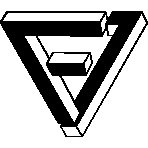
\includegraphics[width=4cm, height=4cm, draft=false] {logo_fi.pdf}
    \vskip4em
    {\begin{spacing}{1}
        \Huge \textbf{An Ahead-of-time\\Compiler for a Subset\\of TypeScript} % XXX: Title
    \end{spacing}}
    \vskip2em
    {\Large \textsc{master's thesis}} % XXX: Type
    \vskip2em
    {\LARGE \textbf{Petr Kubica}} % XXX: Author
    \vfill
    {\hfill\large Brno, 2025} % XXX: Year
\end{center}

\cleardoublepage
\restoregeometry

% XXX: Go edit frontmatter.tex
\section*{Declaration} Hereby I~declare that this paper is my original authorial work, which
I~have worked out on my own. All sources, references, and literature
used or excerpted during elaboration of this work are properly cited
and listed in complete reference to the due source.

\vspace{1cm}
\begin{flushright}
Petr Kubica
\end{flushright}

\vfill\noindent
\textbf{Advisor:} RNDr. Petr Ročkai, Ph.D.   % XXX
% \\\textbf{Konzultant:} nope % XXX
\cleardoublepage

\section*{Acknowledgements} % XXX
I would like to thank everyone who has helped me make this thesis possible, especially my advisor Petr Ročkai for his guidance and advice. I would also like to thank my friends and colleagues, particularly from the ParaDiSe laboratory, for their support. To anyone negatively affected by my lack of time for other work and activities, I apologize and thank you for your understanding. Finally, I would like to thank my family for their support.
\cleardoublepage

\section*{Abstract} % XXX
This thesis describes the design and implementation of an ahead-of-time compiler for a subset of TypeScript. The compiler is implemented as an extension of Jaculus-machine -- a small, embeddable JavaScript runtime environment. The compiler makes use of TypeScript's type annotations to generate more monomorphic code than what is possible by using JavaScript. It can compile parts of an input program to machine code, which can be used to improve its performance. The compiler is then evaluated on several benchmarks and compared to only using an interpreter.

\subsection*{Keywords} % XXX
JavaScript, TypeScript, compiler, ahead-of-time compilation, embedded systems
\cleardoublepage


\setcounter{tocdepth}{2}
\tableofcontents
\pagestyle{plain}

\mainmatter
% XXX: Organise your chapters however the fuck you like
\chapter{Implementation}

The compilation pipeline consists of multiple phases. The input is the content of a single TypeScript file, and the output is runnable JavaScript code with stubs referring to generated native functions.


\section{Parser}

\todo{tokenization}
The first phase of the compilation pipeline involves parsing the input source code. The TypeScript code is converted to an abstract syntax tree (AST) using a recursive descent parser. The design of the parser is inspired by the parser described in the book \textit{Crafting Interpreters}\cite{craftinginterpreters}.

Recursive descent parser is a top-down parser from the family of LL parsers. It is usually implemented by transforming each grammar rule into a function. When a function for a rule is called, it tries to match the input against the rule by recursively calling the functions for its sub-rules.

While recursive parsers are easy to implement and understand, they are not able to parse all grammars. In particular, they cannot parse grammars with left recursion. Because the language grammar, as described in Section \ref{lang:grammar}, is left recursive slight modifications to the grammar and the algorithm are needed.

Infix binary expressions are a case of left recursion in the grammar. They are instead parsed using a cover grammar which is later refined into the correct expression tree. In general, a cover grammar is a more general grammar which is easier to parse but may not produce an equivalent parse tree. The cover grammar is then refined into the correct parse tree using a separate algorithm. The cover grammar used for parsing infix binary expressions is defined as follows:

\todo{fix typesetting iteration}
\GrammarRule[BinaryExpression]{}{
    \nonterminal[UnaryExpression]{}{} \gramiter{\nonterminal[InfixBinaryOperator]{}{} \nonterminal[UnaryExpression]{}{}}
}

The result is a flat representation of the expression without regard to the operator precedence and associativity. It is then refined to the correct expression tree using Shunting Yard algorithm\cite{algol60}.

Another case of left recursion in the grammar are the non-terminals \nonterminal[MemberExpression]{}{} and \nonterminal[CallExpression]{}{}. In both cases, there are multiple productions with left recursion. Fortunately, all of these productions represent a repeated application of a rule. Therefore, they can be parsed iteratively and then transformed into a correct AST. The non-left recursive productions are always applied first, and the left recursive productions are applied in a loop until no more productions can be applied. The grammar for these two non-terminals is defined as follows:

\GrammarRule[MemberExpression]{Yield, Await}{
    \nonterminal[SuperProperty]{?Yield, ?Await}{} \\
    \nonterminal[MetaProperty]{}{} \\
    \nonterminal[PrimaryExpression]{?Yield, ?Await}{} \\
    \terminal{new} \nonterminal[MemberExpression]{?Yield, ?Await}{} \nonterminal[Arguments]{}{} \\
    \nonterminal[MemberExpression]{?Yield, ?Await}{} \terminal{[} \nonterminal[Expression]{?Yield, ?Await}{} \terminal{]} \\
    \nonterminal[MemberExpression]{?Yield, ?Await}{} \terminal{.} \nonterminal[IdentifierName]{}{} \\
    \nonterminal[MemberExpression]{?Yield, ?Await}{} \terminal{.} \nonterminal[PrivateIdentifier]{}{} \\
    \nonterminal[MemberExpression]{?Yield, ?Await}{} \nonterminal[TemplateLiteral]{}{}
}

\GrammarRule[CallExpression]{Yield, Await}{
    \nonterminal[CoverCallExpressionAndAsyncArrowHead]{?Yield, ?Await}{} \\
    \nonterminal[SuperCall]{?Yield, ?Await}{} \\
    \nonterminal[ImportCall]{?Yield, ?Await}{} \\
    \nonterminal[CallExpression]{}{} \nonterminal[Arguments]{}{} \\
    \nonterminal[CallExpression]{}{} \terminal{[} \nonterminal[Expression]{?Yield, ?Await}{} \terminal{]} \\
    \nonterminal[CallExpression]{}{} \terminal{.} \nonterminal[IdentifierName]{}{} \\
    \nonterminal[CallExpression]{}{} \terminal{.} \nonterminal[PrivateIdentifier]{}{} \\
    \nonterminal[CallExpression]{}{} \nonterminal[TemplateLiteral]{}{}
}

The remaining left recursive productions represent simple lists of items and can be, again, parsed iteratively. These non-terminal are: \nonterminal[FormalParameters]{}{}, \nonterminal[Expression]{}{} (comma operator), \nonterminal[LexicalDeclaration]{}{}, \nonterminal[VariableDeclaration]{}{}, \nonterminal[Arguments]{}{}, and \nonterminal[StatementList]{}{}.


\section{Generating the intermediate representation}

After parsing the input source code, the compiler generates an intermediate representation (IR) of the program. The IR is described in detail in Chapter \ref{ir}.

The IR generator traverses the AST and collects all top-level function declarations. From these functions, those suitable for compilation are selected for further processing. The selected functions are then compiled to the IR.

Every function in the AST consists of two parts: a signature and a body. First, the IR generator iterates over all function declarations and creates a list of all possibly compilable functions. In this step, a function is considered compilable if the function signature contains type annotations for all parameters and the return type. The list allows the generator to determine which functions are to be compiled and to insert native calls in relevant places. Then, the function bodies are processed independently on a per-function basis. If compilation of one of these functions fails, the entire compilation process fails with a \texttt{SyntaxError} exception and the input program cannot be executed.

The statements in the function body are recursively traversed by the compiler and the AST is transformed into the intermediate representation described in Chapter \ref{ir}.

The IR generator is implemented as a number of functions which describe the generation process for different AST nodes. These functions keep track of the context of IR generation, in particular, lexical and variable declarations and their scopes, the active basic block, break and continue targets, and the rest of the CFG that is being created.\todo{?}

There are two kinds of AST nodes that generate a part of the IR code -- statements and expressions. When an AST node is being processed, all of its children get processed recursively. In the case of expressions, the sub-nodes have a value result, which may be used by the parent node in some way. The results can have different value types and can be used in different ways. Some may be used as assignment targets (\textit{l-values}) and some may be only used as value operands in another expression (\textit{r-values}). When l-values are to be used as value operands in another expression, they first have to be evaluated (their value is acquired).

The resulting value type of some AST node can not be determined by the node type alone, and depends on the subtree of the node. For example, a \nonterminal[PrimaryExpression]{}{} node may represent a variable (an l-value) or a literal (an r-value). The IR generator therefore first generates the IR code for the sub-nodes and only then determines the value type of the node.

Sometimes, the final value type of evaluated sub-node may be incompatible with what the parent node expects. In these cases, the input code contains syntax error, because static semantics of the language are violated. The IR generator will then throw a \texttt{SyntaxError} exception and abort the compilation process.

When a value is saved into an IR register, its reference count needs to be updated. This operation is implemented by a \texttt{Dup} instruction which is emitted. The reference count needs to be decreased after the value is no longer needed. To avoid analyzing the code and finding the correct places to perform this task, the value is saved using the \texttt{PushFree} instruction and the reference count is decreased before returning from the function.

The process of generating the IR code itself can be viewed as two simple cases -- linear code, and branching code. Generating linear code is trivial, as the respective AST nodes are simply replaced by their counterparts consisting of IR instructions. These can be directly emitted to the currently active basic block.

When generating branching code, the active basic block has to be split into two parts -- entry, and exit. The entry block contains the original code without a terminator instruction while the exit block retains only the terminator instruction. The branching code is then simply emitted into the entry block and a number of newly created blocks for all new paths. Paths that do not terminate, or contain non-linear\todo{check} control flow (i.e., \texttt{break} or \texttt{continue} statements) must all converge to the exit block.

\subsection{Examples of IR generation}

\todo{show the IR-gen of some significant AST nodes -- linear expression, if, for, short-circuit expression, terminating statement}

\subsection{Runtime requirements of IR function}\todo{find a better title}\label{subsec:irruntime}

There are very few requirements on how a function represented by the intermediate representation should behave. The values in IR registers can be stored in any way, be it in CPU registers, in stack memory, or in a different way. There is also no standardized calling convention. The execution environment must only arrange for the function arguments to be passed to the correct IR registers, and the return value to be passed back to the caller.\todo{move to IR chapter?}

A function in the IR requires access to the instance of the JavaScript interpreter it runs under. To implement the \texttt{PushFree} instruction, it also needs a secondary stack (or another container) for storing all values that need to be freed at exit.


\section{Compiler backend}

The compiler relies on the MIR compiler backend to perform register allocation, code generation, and optimization of the machine code. MIR generates functions with a standard calling convention for target platform.

The signature of generated functions is not compatible with the signature of functions callable from QuickJS. Therefore, for every compiled function, a companion function with a compatible signature is generated.

The MIR code is generated by simply replacing parts of the IR with the respective MIR representation. Some simple instructions can be replaced by a single MIR instruction, some more complex are replaced by multiple MIR instructions or a function call.

The final, native, functions require a runtime context, as described in Section \ref{subsec:irruntime}. The context primarily contains a pointer to an instance of the JavaScript interpreter. It also contains a secondary stack used by the \texttt{PushFree} instruction. Lastly, it stores an information about whether an exception has occurred in the function.

Some instructions and function calls may result in a JavaScript exception. For these, additional checks are inserted into the MIR code. These checks use the exception flag in the runtime context to determine whether an exception has occurred. If an exception occurs, the function returns a default value and the exception flag is set. The caller of the function then checks the exception flag and propagates the exception further up the call stack.

These functions are statically bound to a single JavaScript runtime and can not be shared between multiple runtime instances. This allows the functions to use the same runtime context through a constant pointer that is linked to them at compilation.


\section{Stubs}\label{impl:stubs}

After compiling the functions to native code, they need to be made accessible to the interpreter. The compiled functions are therefore wrapped in JavaScript function objects (stubs) which, when called from JavaScript, perform a native call to the compiled function. They are then defined as properties of JavaScript's global object\footnotemark[1] with unique identifiers.

\footnotetext[1]{In JavaScript, a global object is a special object \texttt{globalThis} which is globally accessible from an execution context (i.e., including different modules). Properties of the global object are a part of the lexical scope, and one of its functions is to provide intrinsic objects and values to the execution environment.}

New JavaScript source code is also generated. In this source code, the original declarations of compiled functions are replaced by references to the stubs, and by comments with the original function's source code.

JavaScript applies declaration and value hoisting on function declarations. This means that in a standard JavaScript program, it is possible to reference and use a function before it is declared. In the newly generated code, we can only replicate this behavior by declaring a new function which would call the stub function. Declaring a new function would result in another level of indirection in every call of this function and induce unnecessary overhead.

As maintaining JavaScript's behavior is, in this case, not feasible without modifying the underlying interpreter, we have elected to change the behavior instead. For declaring the aliases for the stub functions, we use a constant lexical declaration (i.e., \texttt{const}). While the runtime semantics is slightly different, its also disallows users from rebinding the same name to a different function (or value). Such behavior would be potentially dangerous, because at compile time functions are statically linked to each other. If the user rebound a function name which was referenced from a different compiled function, they might expect a change in behavior of the compiled function which would, however, not happen. By declaring the function reference as \texttt{const}, such code would result in a syntax error instead.


\section{Interpreter}

The newly generated JavaScript code is then executed by the QuickJS interpreter. The interpreter is not modified and is used through the Jaculus-machine abstraction layer. After preprocessing the source code, as described in Section \ref{impl:stubs}, and defining new properties of the JavaScript's global object, the new JavaScript code is executed as normal.

\section{Integration with Jaculus-machine}

Jaculus-machine uses a modular approach which allows the programmer to select which modules should be a part of a JavaScript runtime (called \textit{Machine}). Jaculus-machine calls these modules \textit{MFeatures}. The configuration of a selected set of MFeatures is performed at compile time which allows the individual MFeatures to interact with one another without significant overhead caused by dynamic bindings.

The compiler implementation is provided as a single MFeature, which provides a method \texttt{eval} for executing input source code. The source code is always processed by the compiler and the generated code is executed.


\backmatter
\chapter{Literature}
\begingroup
\raggedright
\printbibliography[heading=none]
\endgroup

\ifoptiondraft{\listoftodos}

\end{document}
